% The benchmark schematic occupies one column with symbolic constraints.
\begin{figure}[t]
\centering
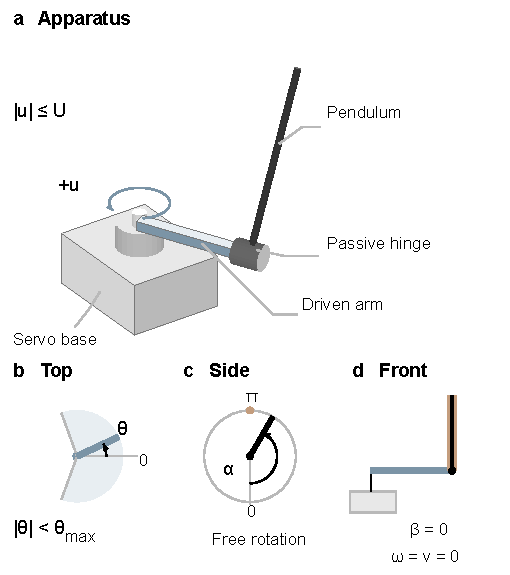
\includegraphics[width=\columnwidth]{figures/rotary-pendulum-geometry/figure-2-rotary-pendulum.pdf}
\caption{Rotary-pendulum apparatus and benchmark requirements.
(a) The servo drives the blue horizontal arm; its end hinge supports a passive rod with rotation axis parallel to the arm.
(b) Top view: the unwrapped arm angle $\theta$ is measured from a fixed reference, and positive shaft torque $u$ increases $\theta$. Prescribed hard design limits are $|\theta|<\theta_{\max}$ and $|u|\le U$, with $\theta_{\max},U>0$.
(c) Side view: the rod rotates freely in the arm-normal vertical plane; $\alpha=0$ is downward and $\alpha=\pi$ is upright.
(d) Front view: ideal upright rest has $\beta=\operatorname{wrap}(\alpha-\pi)=0$ and $\omega=\nu=0$, where $\omega=\dot\theta$ and $\nu=\dot\alpha$ are angular speeds, with wrapping to $[-\pi,\pi)$. The apparatus is schematic. Exact design limits and the ideal rest reference are shown; numerical penalties and finite-tolerance assessment are specified separately in the text.}
\label{fig:rotary-pendulum-geometry}
\end{figure}
